%http://texblog.org/2011/09/09/10-ways-to-customize-tocloflot/

%Автоматически вписывать картинки в ширину страницы:
%\includegraphics[maxwidth=\linewidth]{foobar}

\documentclass[11pt,a4paper,notitlepage]{report}
\makeatletter
\newcommand*{\toccontents}{\@starttoc{toc}}
\makeatother
%\usepackage{pscyr}
\usepackage[utf8]{inputenc}
%\renewcommand{\rmdefault}{ftm}
\renewcommand{\rmdefault}{CMR}
\usepackage[russian]{babel}

\pagestyle{plain} % нумерация страниц вкл.

%\setmainfont{Имя шрифта}
%http://tex.stackexchange.com/questions/181183/combine-usepackagetimes-and-fontspec-setmainfont
%http://andreyolegovich.ru/PC/LaTeX.php#base
\usepackage{amsmath}
\usepackage{graphicx}
\usepackage{pdfpages}
\usepackage{comment}
\usepackage{textcomp}
\usepackage{wrapfig}
\usepackage{sectsty}
\usepackage{lipsum}
\usepackage{fancyhdr}
\usepackage{datetime}
%\allsectionsfont{\centering}
\chapterfont{\centering}
\usepackage[T2A]{fontenc}
\usepackage{lscape}
\usepackage{makecell}
\usepackage{multicol}
\usepackage{titlesec}
\usepackage{floatrow}
\usepackage{float}
\usepackage{caption}


\graphicspath{{img/}}

%*****************************************************
% Часто требуется, чтобы номер рисунка содержал в себе номер главы (вроде Рис. 1.1). Чтобы была сделана нумерация по главам, достаточно изменить счётчик рисунков в преамбуле документа вот так:
\renewcommand{\thefigure}{\thesection.\arabic{figure}}
%*****************************************************

%*****************************************************
%Если вас не устраивает вид подрисуночной подписи (например, вместо "Рис. 1:" необходимо "Рис. 1 --- "), используйте пакет caption. В частности, для установки тире в качестве разделителя, вставьте в преамбулу документа следующий код: 
\RequirePackage{caption}
\DeclareCaptionLabelSeparator{defffis}{ --- }
\captionsetup{justification=centering,labelsep=defffis}
%*****************************************************

%\usepackage[colorlinks=true,linkcolor=blue]{hyperref}

%*****************************************************
%Как сделать, чтобы уравнения нумеровались независимо по главам в LaTeX?
%В преамбуле
\makeatletter \@addtoreset{equation}{section} \makeatother 
\makeatletter \@addtoreset{figure}{section} \makeatother 
%*****************************************************

\addto\captionsrussian{
	\def\figurename{Рисунок}
}


\usepackage[hypcap]{caption}

%*****************************************************
% Начинать секции с новой страницы
%\usepackage{titlesec}
%\newcommand{\sectionbreak}{\clearpage}
%*****************************************************


%*****************************************************
%Чтобы в генерированном PDF работали гиперссылки, то надо подключить модуль hyperref (и если хотите их разрисовать, то модуль по работе с цветами xcolor):
\usepackage{xcolor}
\usepackage{hyperref}
% Цвета для гиперссылок
\definecolor{linkcolor}{HTML}{012b37} % цвет ссылок
\definecolor{urlcolor}{HTML}{012b37} % цвет гиперссылок
\hypersetup{pdfstartview=FitH,  linkcolor=linkcolor,urlcolor=urlcolor, colorlinks=true}
%*****************************************************

%***************************************************** 
%Для удаления номеров страниц из \listoffigures
\makeatletter
\newcommand{\emptypage}[1]{%
	\cleardoublepage
	\begingroup
	\let\ps@plain\ps@empty
	\pagestyle{empty}
	#1
	\cleardoublepage}
\makeatletter
%*****************************************************


\setcounter{secnumdepth}{3}
%\usepackage{enumitem}
\usepackage[shortlabels]{enumitem}
\setlist[enumerate]{leftmargin=*,align=left,label=\thesubsection.\arabic*.}
%\usepackage{enumerate}

\usepackage{lastpage} 

\usepackage{longtable}




%\renewcommand{\rmdefault}{ftm}
\renewcommand{\rmdefault}{cmr}
\renewcommand{\thesection}{\arabic{section}}
%\usepackage{enumitem}
%%% Страница
%\usepackage{extsizes} % Возможность сделать 14-й шрифт
\usepackage{geometry} % Простой способ задавать поля
\geometry{top=15mm}
\geometry{bottom=10mm}
\geometry{left=10mm}
\geometry{right=10mm}

%*****************************************************
%Here is how you can increase the space between the number and the caption in your \listoffigures. Add the following two lines before your \begin{document}:
\usepackage{tocloft}
\setlength{\cftfignumwidth}{3em}
%With the tocloft-package you can control the design of table of contents, figures and tables.
%*****************************************************


\usepackage{svn}

\pagestyle{fancy}
%\fancyfoot[]{вер. 1.05}
\fancyfoot[]{Страница \thepage \; из \pageref{LastPage}}
\renewcommand{\headrulewidth}{0pt}
\renewcommand{\footrulewidth}{0pt}
\setlength\headheight{80.0pt}
\addtolength{\textheight}{-80.0pt}
\chead{
\includegraphics[width=\textwidth]{img/log1o.png}}
\cfoot{
\includegraphics[width=\textwidth]{img/foot.png}}





%*****************************************************
%Номера страниц, включающие номер главы
\usepackage[auto]{chappg} %%% this is to set the page numbers as Chapter-Page.
%*****************************************************



\newdate{date}{18}{04}{2016}
\date{\displaydate{date}}
%Increase the value of tocdepth and secnumdepth. The tocdepth value determines to which level the sectioning commands are printed in the ToC (they are always included in the .toc file but ignored otherwise). The secnumdepth value determines up to what level the sectioning titles are numbered. They are LaTeX counters and you can set them using 
\setcounter{tocdepth}{1}
\setcounter{secnumdepth}{4}



%\titlespacing\section{0pt}{12pt plus 4pt minus 2pt}{0pt plus 2pt minus 2pt}
%\titlespacing{\subsection}{0pt}{\parskip}{-\parskip}

\begin{document}
	
\begin{flushright}
\end{flushright}

\vspace{\baselineskip}
\vspace{\baselineskip}
\vspace{\baselineskip}
\vspace{\baselineskip}

\begin{center}
Инструкция\\
по настройке электронной почты \\
на планшете с Android \tiny{вер. 0.1} 
\end{center}


\begin{multicols}{2}
\flushleft г. Новосибирск
\flushright \displaydate{date} 
\end{multicols}

\toccontents

%\pagenumbering{roman}
%\tableofcontents
%\listoffigures
%\listoftables
%\clearpage
%\pagenumbering{arabic}
%czxc
\addtocontents{toc}{~\hfill\textbf{Стр.}\par}
%\section{Добавление аккуаунта эл.почты}
Для добавления аккаунта эл.почты необходимо выполнить следующие:
\begin{enumerate}[\thesection .1]
\item  Зайти в меню планшета (рис.\ref{pic:pic_1}):
 \begin{figure}[H]
 	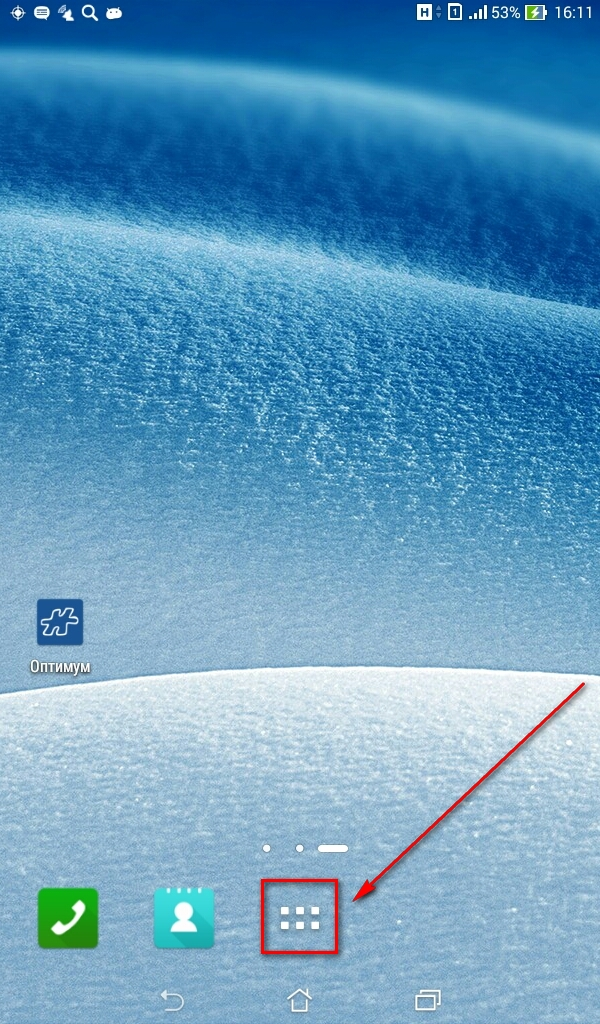
\includegraphics[width=0.3\linewidth]{pic_1.jpg} 
 	\caption{Меню}\label{pic:pic_1}
 \end{figure}
\item Выбрать и нажать на значок "Настройка" планшета (рис.\ref{pic:pic_2}):
 \begin{figure}[H]
 	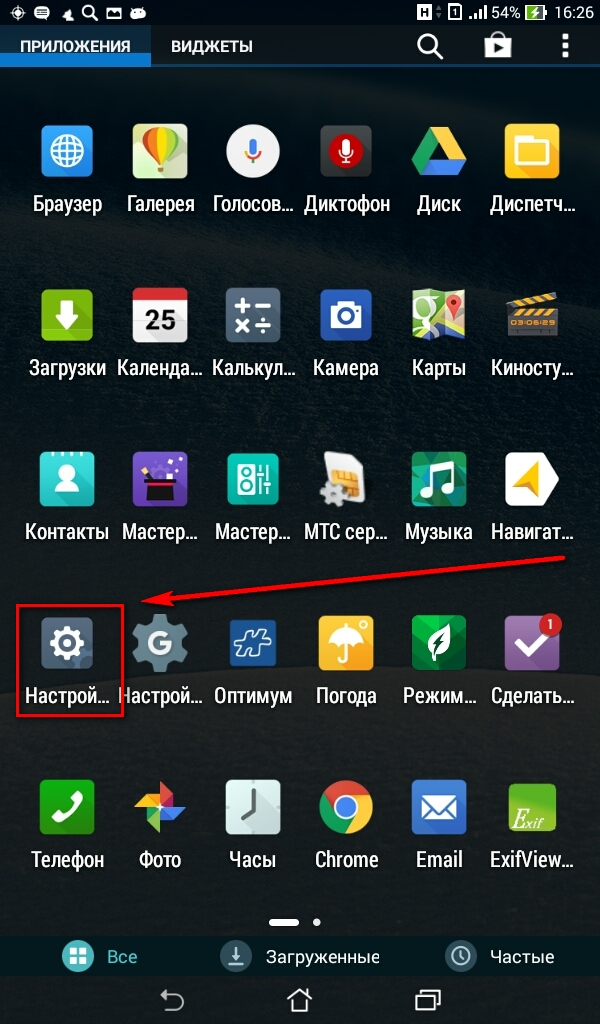
\includegraphics[width=0.3\linewidth]{pic_2.jpg} 
 	\caption{Настройка}\label{pic:pic_2}
 \end{figure}
\item Откроется окно настроек планшета (рис.\ref{pic:pic_3}):
 \begin{figure}[H]
 	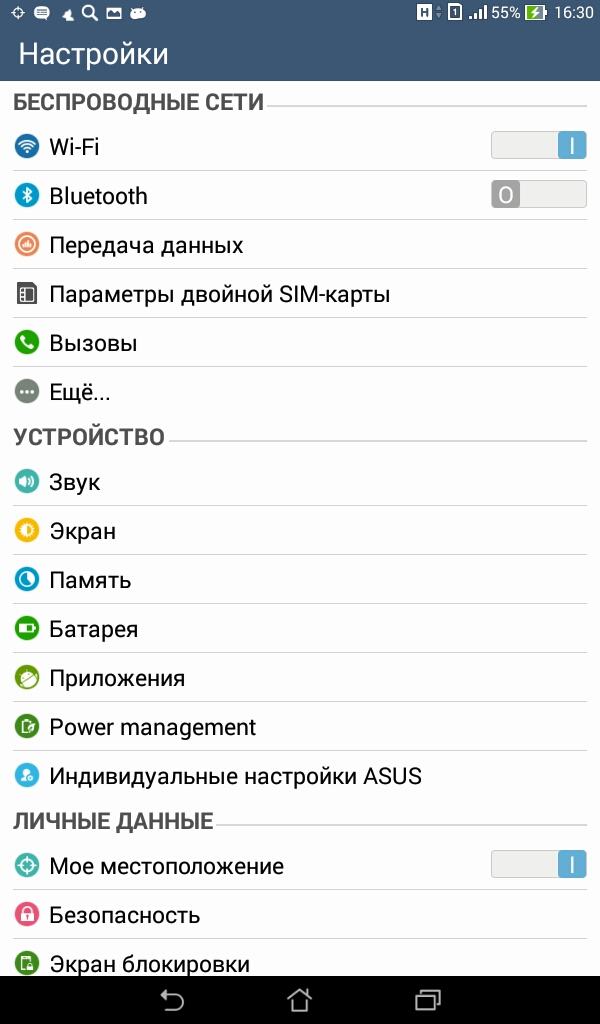
\includegraphics[width=0.3\linewidth]{pic_3.jpg} 
 	\caption{Настройки планшета}\label{pic:pic_3}
 \end{figure}
 \item "Пролистать" список вниз до появления пункта "Добавить аккаунт" (рис.\ref{pic:pic_4}):
  \begin{figure}[H]
  	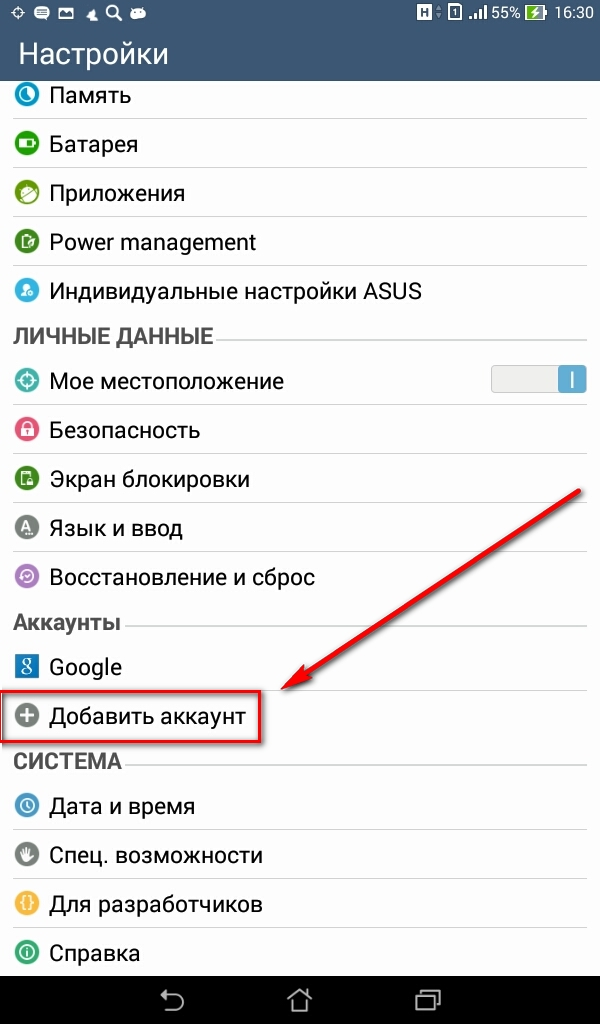
\includegraphics[width=0.3\linewidth]{pic_4.jpg} 
  	\caption{Пункт "Добавить аккаунт"}\label{pic:pic_4}
  \end{figure}
\item Выбрать его, затем найти и выбрать "Google" (рис.\ref{pic:pic_5}):
  \begin{figure}[H]
  	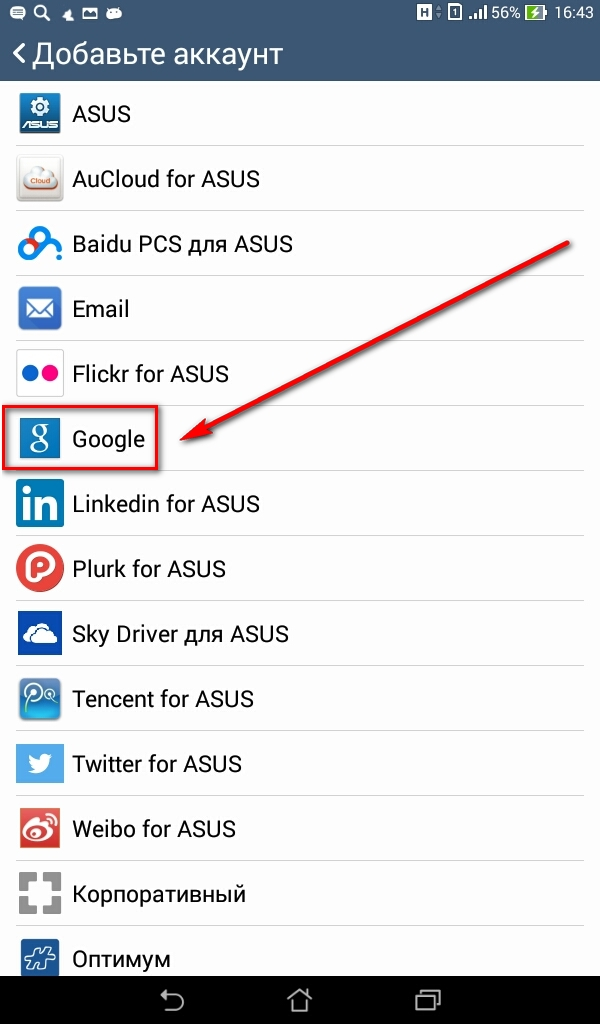
\includegraphics[width=0.3\linewidth]{pic_5.jpg} 
  	\caption{"Google"}\label{pic:pic_5}
  \end{figure}
  
\begin{itemize}[topsep=0pt, itemsep=-0.5ex]
	\item сбор дебиторской задолженности у клиентов
	\item поиск новых клиентов
	\item экстренной ситуации, требующей незамедлительного присутствия торгового представителя.
\end{itemize}
\item Торговый представитель может принимать заявки по телефону от торговых точек, не указанных в маршрутном листе соответствующего рабочего дня.
%\item Рабочий день торгового представителя (согласно данным GPRS), а именно, посещение последней торговой точки согласно маршрутному листу, заканчивается в 16:30.
\end{enumerate}% Регистрация почты
%\section{Настройка эл.почты на планшете}
\begin{enumerate}[\thesection .1]
	\begin{figure}[H]
		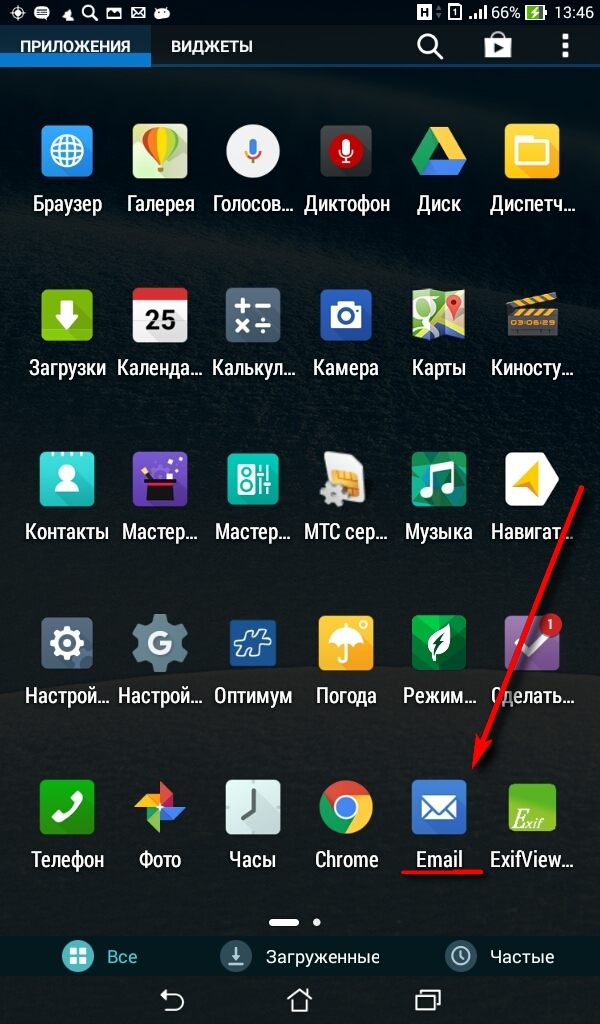
\includegraphics[width=0.3\linewidth]{pic_16.jpg} 
		\caption{Меню}\label{pic:pic_16}
	\end{figure}
	\item  Необходимо зайти в меню планшета найти и запустить приложение "Email" (рис.\ref{pic:pic_16}), в зависимости от версии Android и модели планшета иконка приложения может отличатся от представленной на рисунке. 
	\newpage 
	
	\begin{figure}[!h]
		\begin{floatrow}
			\ffigbox{\caption{Выбор провайдера эл.почты}\label{pic:pic_17}}%
			{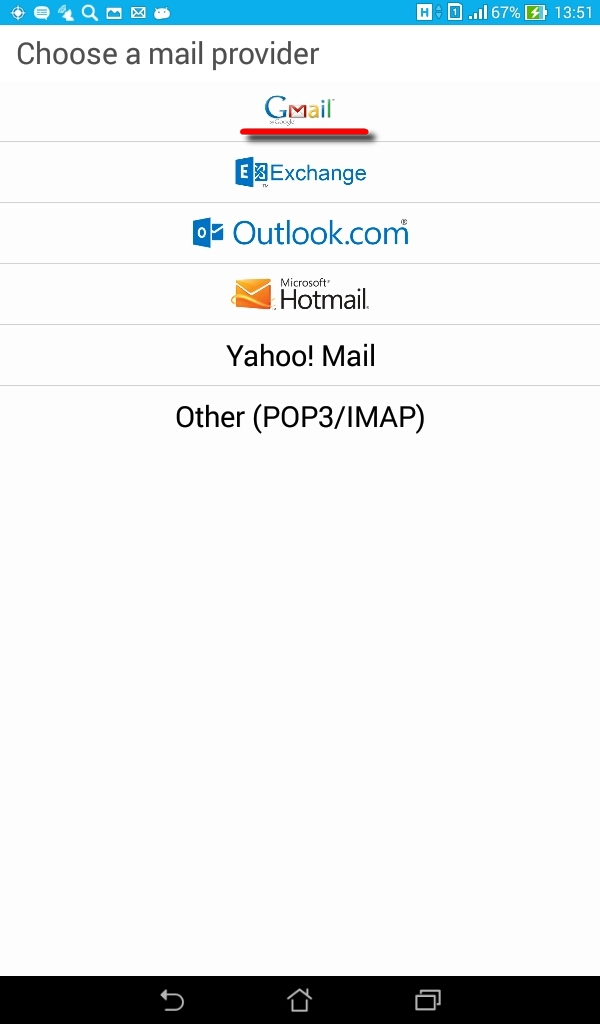
\includegraphics[width=0.58\linewidth]{pic_17.jpg}}
			\ffigbox{\caption{Выбор нужного аккаунта}\label{pic:pic_18}}%
			{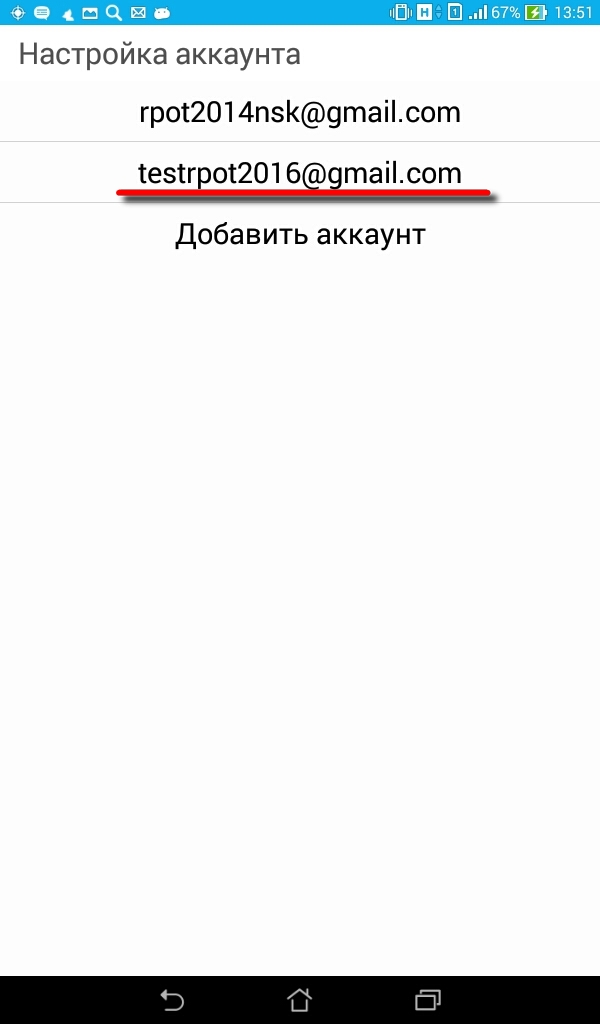
\includegraphics[width=0.58\linewidth]{pic_18.jpg}}         
		\end{floatrow}
	\end{figure}
	
	\item Выбрать нужного провайдера эл.почты, в нашем случае это "Gmail" (рис.\ref{pic:pic_17}):
	\item Из предложенного списка выбрать нужный аккаунт (рис.\ref{pic:pic_18}):

	
	\begin{figure}[!h]
		\begin{floatrow}
			\ffigbox{\caption{Ожидание входа}\label{pic:pic_19}}%
			{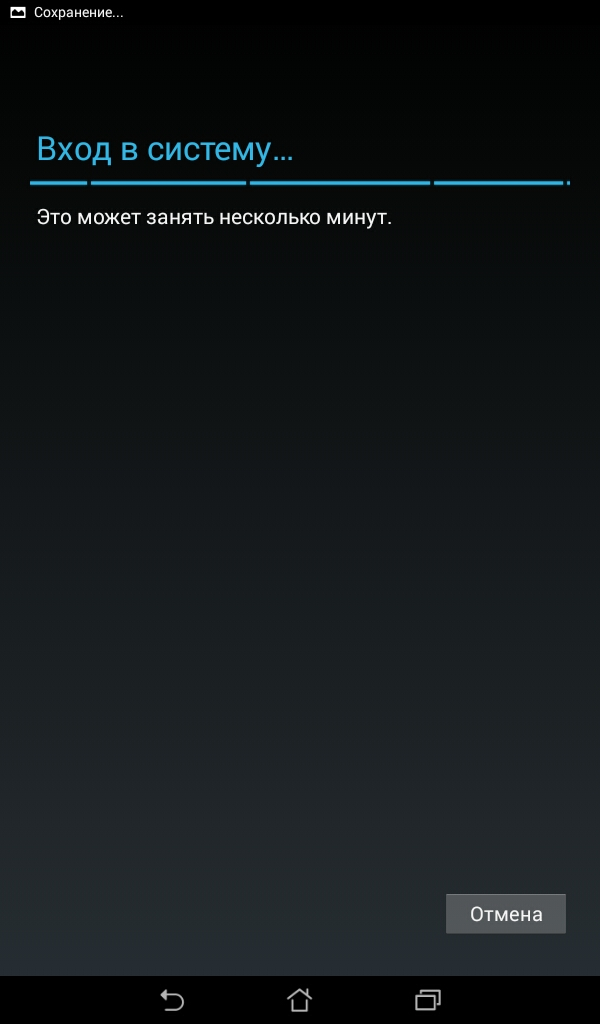
\includegraphics[width=0.58\linewidth]{pic_19.jpg}}
			\ffigbox{\caption{Подтверждение разрешений}\label{pic:pic_20}}%
			{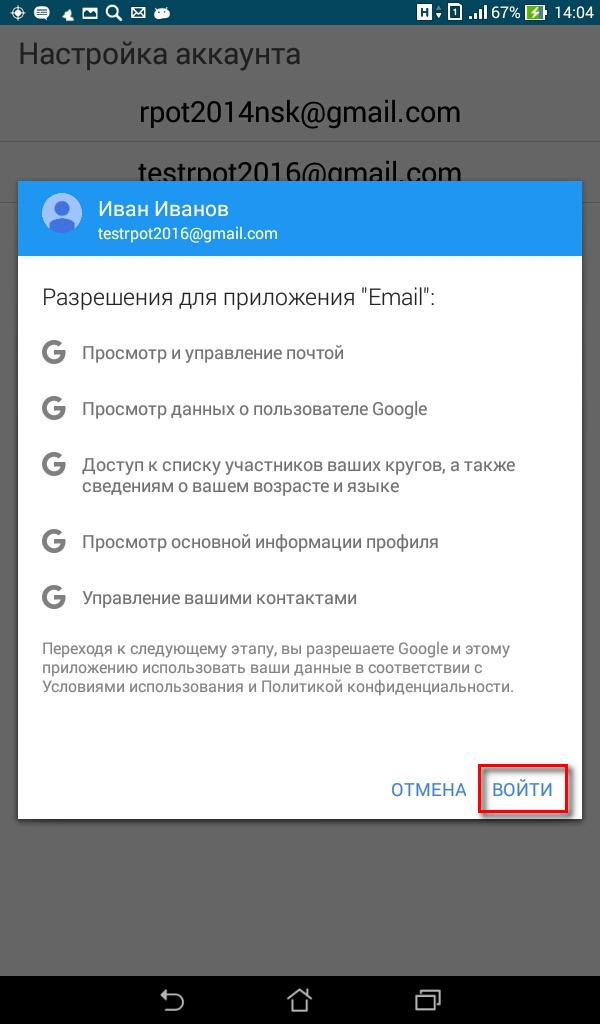
\includegraphics[width=0.58\linewidth]{pic_20.jpg}}         
		\end{floatrow}
	\end{figure}
	
	\item Далее некоторое время ожидаем входа в систему (рис.\ref{pic:pic_19}), после чего на запрос о разрешениях отвечаем "Войти" (рис.\ref{pic:pic_20}).


	\newpage 
	
	\begin{figure}[!h]
		\begin{floatrow}
			\ffigbox{\caption{Проверка настроек сервера}\label{pic:pic_21}}%
			{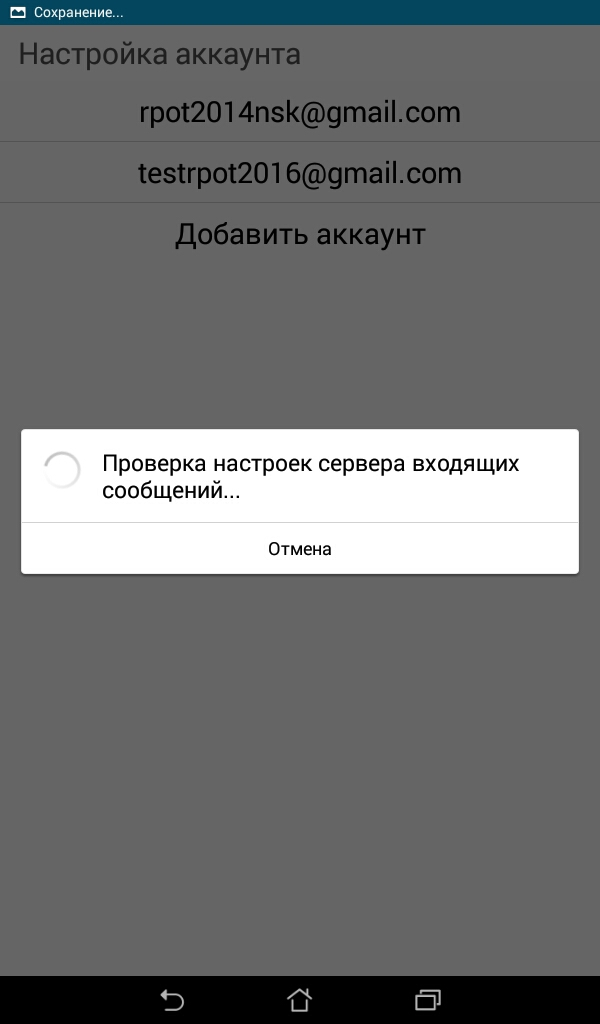
\includegraphics[width=0.58\linewidth]{pic_21.jpg}}
			\ffigbox{\caption{Настройки параметров аккаунта}\label{pic:pic_22}}%
			{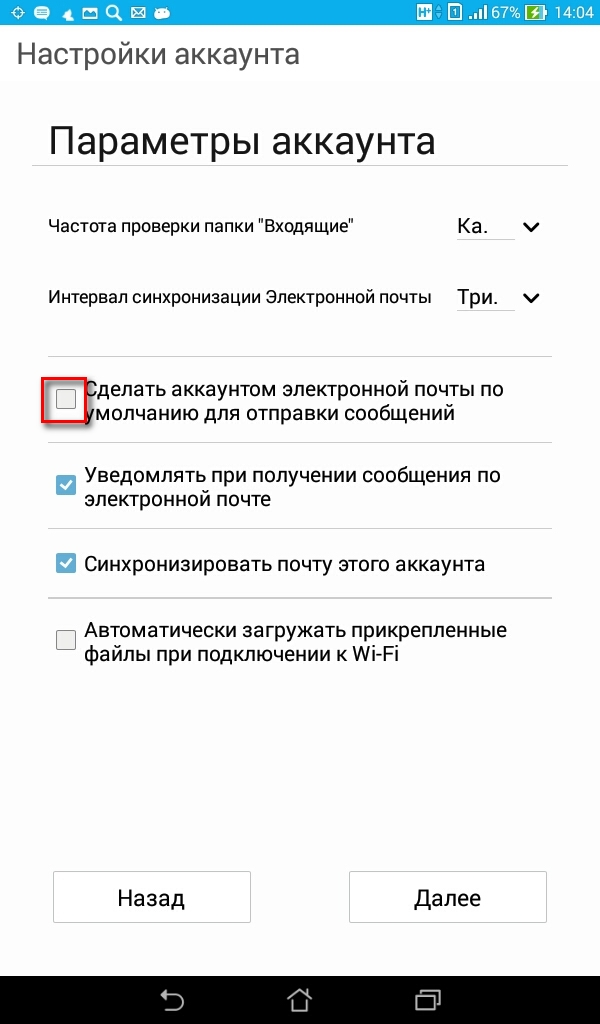
\includegraphics[width=0.58\linewidth]{pic_22.jpg}}         
		\end{floatrow}
	\end{figure}
	
	\item Дожидаемся пока Google проверит корректность настроек сервера (рис.\ref{pic:pic_21}) и затем проставив в настройка аккаунта галку "Сделать аккаунтом электронной почты по умолчанию"  (рис.\ref{pic:pic_22}), нажимаем "Далее"
	
	
	\begin{figure}[!h]
		\begin{floatrow}
			\ffigbox{\caption{Настроенный аккаунт}\label{pic:pic_23}}%
			{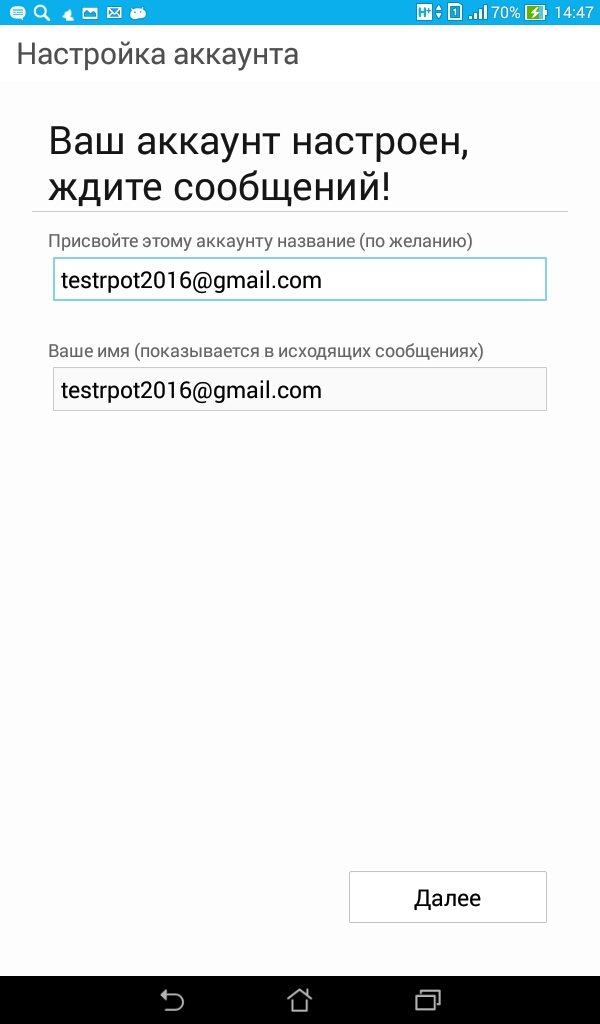
\includegraphics[width=0.58\linewidth]{pic_23.jpg}}
			\ffigbox{\caption{Синхронизация почты}\label{pic:pic_24}}%
			{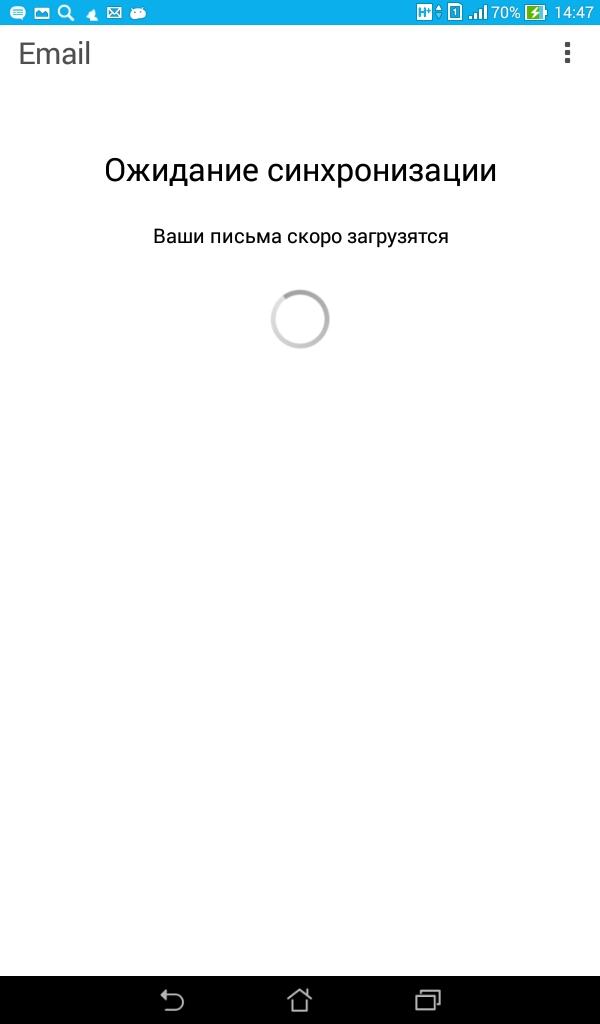
\includegraphics[width=0.58\linewidth]{pic_24.jpg}}         
		\end{floatrow}
	\end{figure}
	
	\item Читаем сообщение о том, что на аккаунт настроен, при желании корректируем доступные данные (рис.\ref{pic:pic_23}), дожидаемся проверки почты... (рис.\ref{pic:pic_24}).


\newpage
\begin{figure}[H]
	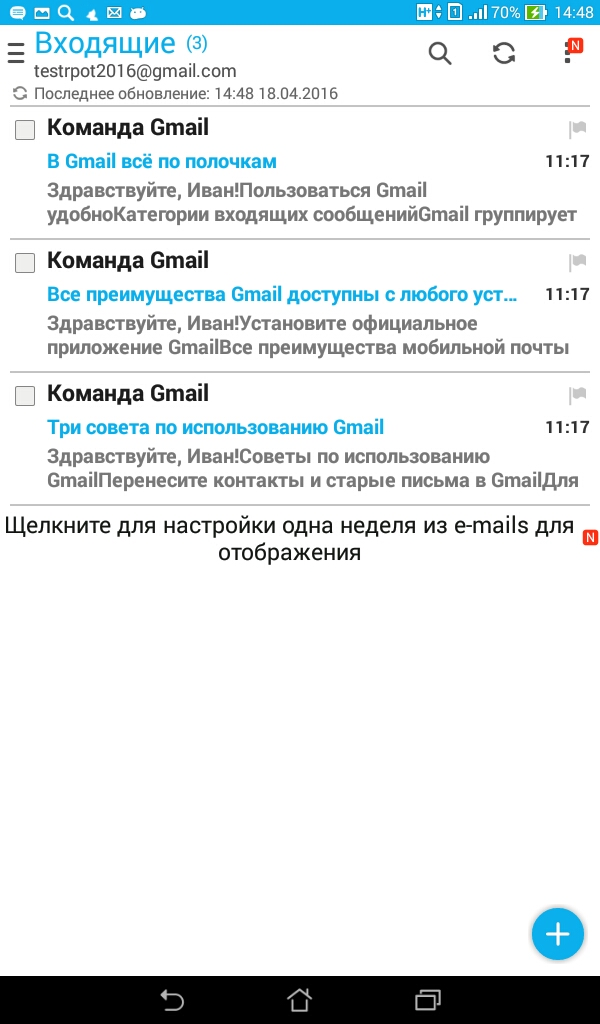
\includegraphics[width=0.3\linewidth]{pic_25.jpg} 
	\caption{Почтовый ящик}\label{pic:pic_25}
\end{figure}
\item Ваша программа электронной почты настроена. (рис.\ref{pic:pic_25}):


\end{enumerate}% Последовательность работы торгового представителя с планшетным устройством
%\section{Введение}
\begin{enumerate}[\thesection .1]
\item Внимание, все скриншоты были выполнены на планшете ASUS с версией Android 4.3. Так что, приведённые картинки могут отличаться  от конкретных планшетов торговых представителей, на которых будет происходить настройка электронной почты. В случае неясности или возникновении проблем при добавлении аккаунта электронной почты, торговый представитель связывается с службой поддержки.
\end{enumerate}% Работа в торговой точке
%\section{Предоставление отчета о деятельности торгового агента.}
Аналитик – координатор отдела прямых продаж ООО «Регионпродоптторг» на ежедневной основе, по факту окончания рабочего дня торгового представителя (до 18:00 текущего дня)  формирует «Отчёт о деятельности агента» с программы 1С ООО «Регионпродоптторг» за текущий день (форма документа в Приложении № 1 к настоящему Регламенту) и направляет данный сформированный отчёт на электронный адрес следующим лицам:
\begin{itemize}[topsep=0pt, itemsep=-0.5ex]
	\item Супервайзеру отдела городских продаж ООО «Торговый Дом «Солнечные Продукты».
	\item Региональному менеджеру по продажам ООО «Торговый Дом «Солнечные продукты».
\end{itemize}

%\input{tex/p5.tex}
%\input{tex/p6.tex}
%\input{tex/p8.tex}% Дебиторка
%\input{tex/p9.tex}% Полная синхронизация
%\input{tex/p10.tex}% Ввод временных координат
%\input{tex/p7.tex}% Закрытие программы
%\input{tex/p11.tex}% Внеплановый визит
%\input{tex/p12.tex}%Описание раздела <<Визиты>>
%\input{tex/p13.tex}%Описание раздела <<Документы>>
%\input{tex/p14.tex}%Описание раздела <<Клиенты>>
%\input{tex/p15.tex}%Описание раздела <<Товары>>
%\input{tex/p16.tex}%Описание раздела <<Баланс>>
%\input{tex/p17.tex}%Описание раздела <<Настройки>>
%\input{tex/p18.tex}%Описание раздела <<Принципы управления>>
\cleardoublepage
\addcontentsline{toc}{section}{\listfigurename}
%\pagestyle{empty}
%\listoffigures
%\cleardoublepage
\begingroup
\renewcommand\numberline[1]{}
%\listoffigures\thispagestyle{empty} \newpage
\emptypage\listoffigures\thispagestyle{empty} \newpage
\endgroup
%\listoffigures\thispagestyle{empty} \newpage
\end{document}

%enumerate latex \subsection
%
%If you need it only for a few enumerate environments, instead of setting globally
%
%\setlist[enumerate]{leftmargin=*,align=left,label=\thesubsection.\arabic*.}
%
%use these settings locally by issuing
%
%\begin{enumerate}[leftmargin=*,align=left,label=\thesubsection.\arabic*.]
%	
%	Note that you may need to load enumitem with the shortlabels option
%	
%	\usepackage[shortlabels]{enumitem}
%	
%	if you have already customized enumerate lists.


%http://tex.stackexchange.com/questions/227005/alignment-of-enumerate-numbered-by-subsection-and-the-existing-text

%http://tex.stackexchange.com/questions/1126/include-section-number-in-list-number

%latex list enumerate \subsection number

%\begin{wrapfigure}{l}{0.4\linewidth}
%\includegraphics[width=0.8\linewidth]{img/scr4.jpg} 
%\caption{Меню синхронизация}\label{pic:pic4}
%\end{wrapfigure}

%
%Соглашусь с тов. Const, что при хитром размещении картинок на титульном листе, может оказаться проще использовать точное позиционирование, например, посредством tikz: что-то вроде
%
%\begin{tikzpicture}
%\node at (0,0){\includegraphics{картинка}};
%\node at (1,0){\includegraphics{картинка}};
%\end{tikzpicture}